\documentclass[aspectratio=169,12pt]{beamer}

% ── Packages ──────────────────────────────────────────────────────────────────
\usepackage[utf8]{inputenc}
\usepackage[T1]{fontenc}
\usepackage{lmodern}
\usepackage{amsmath,amssymb,amsthm}
\usepackage{bm}
\usepackage{graphicx}
\usepackage{tikz}
\usetikzlibrary{arrows.meta,positioning,shapes.geometric,fit,calc}
\usepackage{pgfplots}
\pgfplotsset{compat=1.18}
\usepackage{booktabs}
\usepackage{listings}
\usepackage{hyperref}
\usepackage{xcolor}
\usepackage{algorithm}
\usepackage{algpseudocode}

% ── Theme ─────────────────────────────────────────────────────────────────────
\usetheme{Madrid}
\usecolortheme{default}
\usefonttheme{professionalfonts}

\definecolor{mlblue}{RGB}{0,82,147}
\definecolor{mlorange}{RGB}{220,100,0}
\definecolor{mlgreen}{RGB}{0,130,70}
\definecolor{mlgray}{RGB}{80,80,80}

\setbeamercolor{structure}{fg=mlblue}
\setbeamercolor{block title}{bg=mlblue,fg=white}
\setbeamercolor{block body}{bg=mlblue!10}
\setbeamercolor{alerted text}{fg=mlorange}
\setbeamercolor{example text}{fg=mlgreen}

% ── Code listings ─────────────────────────────────────────────────────────────
\lstset{
  basicstyle=\ttfamily\footnotesize,
  keywordstyle=\color{mlblue}\bfseries,
  commentstyle=\color{mlgray}\itshape,
  stringstyle=\color{mlgreen},
  numberstyle=\tiny\color{mlgray},
  numbers=left,
  numbersep=5pt,
  breaklines=true,
  frame=single,
  backgroundcolor=\color{black!5},
}

% ── Math macros ───────────────────────────────────────────────────────────────
\newcommand{\R}{\mathbb{R}}
\newcommand{\E}{\mathbb{E}}
\newcommand{\norm}[1]{\left\lVert#1\right\rVert}
\newcommand{\abs}[1]{\left|#1\right|}
\newcommand{\vect}[1]{\bm{#1}}
\newcommand{\mat}[1]{\mathbf{#1}}
\DeclareMathOperator*{\argmin}{arg\,min}
\DeclareMathOperator*{\argmax}{arg\,max}
\DeclareMathOperator{\softmax}{softmax}

% ── Title info ────────────────────────────────────────────────────────────────
\title[Short Title]{Full ML Presentation Title}
\subtitle{Optional Subtitle}
\author[Author]{Author Name}
\institute[Inst.]{Department \\ University / Organization}
\date{\today}

% ── Document ──────────────────────────────────────────────────────────────────
\begin{document}

\begin{frame}
  \titlepage
\end{frame}

\begin{frame}{Agenda}
  \tableofcontents
\end{frame}

% ── SECTION 1 ─────────────────────────────────────────────────────────────────
\section{Motivation}

\begin{frame}{Motivation}
  \begin{columns}[T]
    \begin{column}{0.55\textwidth}
      \begin{itemize}
        \item Why does this problem matter?
        \item Current limitations
        \item Our proposed approach
      \end{itemize}
    \end{column}
    \hfill
    \begin{column}{0.40\textwidth}
      % \includegraphics[width=\textwidth]{figures/motivation.png}
      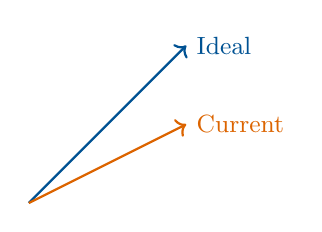
\begin{tikzpicture}
        \draw[mlblue,thick,->] (0,0) -- (2,2) node[right]{\small Ideal};
        \draw[mlorange,thick,->] (0,0) -- (2,1) node[right]{\small Current};
      \end{tikzpicture}
    \end{column}
  \end{columns}
\end{frame}

% ── SECTION 2 ─────────────────────────────────────────────────────────────────
\section{Background}

\begin{frame}{Background}
  \begin{block}{Key Concept}
    Formal definition or important equation:
    \begin{equation}
      f(\vect{x}) = \sigma\!\left(\mat{W}\vect{x} + \vect{b}\right)
    \end{equation}
  \end{block}
  \vspace{0.5em}
  \begin{itemize}
    \item $\mat{W} \in \R^{d_{\text{out}} \times d_{\text{in}}}$ -- weight matrix
    \item $\vect{b} \in \R^{d_{\text{out}}}$ -- bias vector
    \item $\sigma$ -- non-linear activation function
  \end{itemize}
\end{frame}

% ── SECTION 3 ─────────────────────────────────────────────────────────────────
\section{Method}

\begin{frame}{Proposed Method}
  \begin{algorithm}[H]
    \caption{Training Loop}
    \begin{algorithmic}[1]
      \Require dataset $\mathcal{D}$, learning rate $\eta$
      \State Initialize parameters $\theta$
      \For{each epoch}
        \For{each mini-batch $(\vect{x}, y) \in \mathcal{D}$}
          \State $\hat{y} \leftarrow f_\theta(\vect{x})$
          \State $\mathcal{L} \leftarrow \ell(\hat{y}, y)$
          \State $\theta \leftarrow \theta - \eta\,\nabla_\theta\mathcal{L}$
        \EndFor
      \EndFor
    \end{algorithmic}
  \end{algorithm}
\end{frame}

\begin{frame}{Architecture}
  \centering
  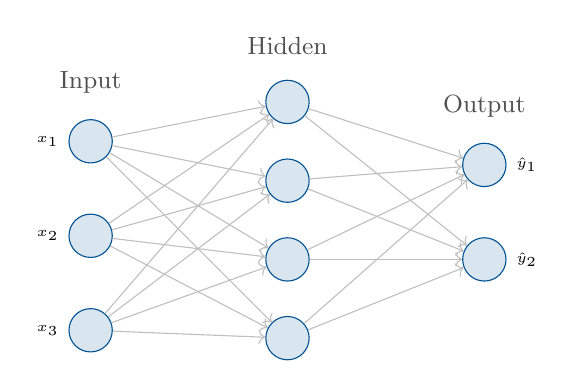
\begin{tikzpicture}[
    node distance=1.4cm,
    neuron/.style={circle,draw=mlblue,fill=mlblue!15,minimum size=0.55cm,inner sep=0},
  ]
    \foreach \i in {1,2,3}
      \node[neuron,label=left:{\tiny $x_\i$}] (in\i) at (0,-\i*1.2) {};
    \foreach \i in {1,2,3,4}
      \node[neuron] (h\i) at (2.5,-\i*1.0+0.3) {};
    \foreach \i in {1,2}
      \node[neuron,label=right:{\tiny $\hat{y}_\i$}] (out\i) at (5,-\i*1.2-0.3) {};
    \foreach \i in {1,2,3}
      \foreach \j in {1,2,3,4}
        \draw[->,gray!50,thin] (in\i) -- (h\j);
    \foreach \i in {1,2,3,4}
      \foreach \j in {1,2}
        \draw[->,gray!50,thin] (h\i) -- (out\j);
    \node[above=0.2cm of in1,mlgray]{\small Input};
    \node[above=0.2cm of h1,mlgray]{\small Hidden};
    \node[above=0.2cm of out1,mlgray]{\small Output};
  \end{tikzpicture}
\end{frame}

% ── SECTION 4 ─────────────────────────────────────────────────────────────────
\section{Experiments}

\begin{frame}{Experimental Results}
  \begin{table}
    \centering
    \caption{Comparison on benchmark dataset}
    \begin{tabular}{lccc}
      \toprule
      \textbf{Method} & \textbf{Accuracy} & \textbf{F1} & \textbf{Params} \\
      \midrule
      Baseline        & 82.3              & 81.1        & 10M \\
      Method A        & 85.7              & 84.9        & 12M \\
      \textbf{Ours}   & \textbf{88.2}     & \textbf{87.6} & 11M \\
      \bottomrule
    \end{tabular}
  \end{table}
\end{frame}

% ── SECTION 5 ─────────────────────────────────────────────────────────────────
\section{Conclusions}

\begin{frame}{Conclusions}
  \begin{block}{Summary}
    \begin{enumerate}
      \item Key finding 1
      \item Key finding 2
      \item Key finding 3
    \end{enumerate}
  \end{block}
  \vfill
  \begin{alertblock}{Future Work}
    \begin{itemize}
      \item Open problem A
      \item Open problem B
    \end{itemize}
  \end{alertblock}
\end{frame}

% ── References ────────────────────────────────────────────────────────────────
\begin{frame}[allowframebreaks]{References}
  \bibliographystyle{apalike}
  \bibliography{references}
\end{frame}

% ── Thank you ─────────────────────────────────────────────────────────────────
\begin{frame}
  \centering
  \Huge\bfseries\color{mlblue} Thank You!\\[1em]
  \normalsize Questions \& Discussion\\[2em]
  \small \texttt{author@institution.edu}
\end{frame}

\end{document}
